\chapter[Gestion des présences]{Gestion des présences\raisebox{.3\baselineskip}{\normalsize\footnotemark}}
\footnotetext{\url{https://github.com/barnabegeffroy/Attendance}}

L'offre de stage\footnote{\href{https://github.com/Dauphine-MIDO/M1-app/blob/master/Stage dev.adoc}{\textcolor{blue}{\underline{Offre de stage: développement agile d’applications web et de bibliothèques open-source}}}} auquel je me suis porté candidat portait initialement sur le développement d'une application gérant la présence des élèves du Master 1 MIAGE en Apprentissage. L'idée de ce projet était de digitaliser les feuilles de présences.

\section{Attendance}

Le projet Attendance avait donc pour but de développer une application web liée à la gestion des présences des élèves. Le serveur HTTP Eclipse Jetty, 

\begin{figure}[!h]
    \begin{center}
    %taille de l'image en largeur
    %remplacer "width" par "height" pour régler la hauteur
    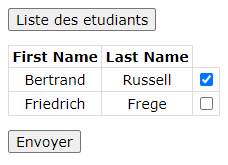
\includegraphics[width=5cm]{assets/attendance.PNG}
    \end{center}
    %légende de l'image
    \caption{Enveloppe d'un son}
\end{figure}

\section{JeSuisEnCours}

Après quelques semaines, nous nous sommes rendus compte que la direction du projet était incompatible avec les exigences administratives. En effet, l'application prévoyait un simple appel du professeur, or l'étudiant doit personnellement attester de sa présence en émargeant un document. Il donc été décidé d'abandonner le projet intiale Attendance pour se tourner vers une application JeSuisEnCours, spécialisée dans la digitalisation les feuilles de présences. 

Le but principal du projet est donc devenu la connexion de l'application JeSuisEnCours aux données de l'université, d'une part, pour accéder aux données (annuaires, emploies du temps,...), d'autre part pour gérer les éléments renvoyés par l'application (absence, justificatif,...).

Malheureursement, la crise sanitaire a fortement ralentit les contacts avec l'équipe de JeSuisEnCours et le projet a finalement été abandonné.